\section{Géométrie des polyèdres}

Un \emph{polyèdre} est un sous-ensemble de $\R^n$ qui peut être écrit comme ${\mathcal P}=\{x \in \R^n |\;  Ax \geq b \}$. Un polyèdre est une
intersection d'un nombre fini d'ensembles convexes et c'est donc un ensemble convexe. Soit
$\mathcal P$ un poly\`edre de
$\R^n$. La solution
$\xopt
\in \R^n$ est une
\emph{solution admissible de base}  de
$\mathcal P$ (pour les poly\`edres, \emph{sommet}, \emph{point extrême} et \emph{solution admissible de base} sont synonymes)
si  $\xopt$ est une solution admissible ($\xopt
\in {\mathcal{P}}$) et s'il y a
$n$ contraintes linéairement indépendantes actives en
$\xopt$. Une solution admissible de base $\xopt$ est \emph{dégénérée}     s'il y a plus de $n$ contraintes actives en
$\xopt$. Deux solutions admissibles de base sont \emph{adjacentes}   si elles partagent $n-1$ contraintes linéairement indépendantes
actives.\\


\newpage



\begin{enumerate}




  \item Soit le poly\`edre défini par les inégalités linéaires

    $
    \begin{array}{rcr}
      x_1+4 x_2-2x_3 & = & 7\\
      2x_2 -3x_3 & \leq & 1\\
      x_2 & \geq & 2\\
      x_3& \geq & 0
    \end{array}
    $

    Le point $(1, 2, 1)$ est-il un sommet du poly\`edre? et le point $(5, 1/2, 0)$?


    \begin{solution}
      $x = (1,2,1)$ est un sommet parce qu'il y a $n = 3$ contraintes linéairement indépendantes serrées et $x \in P$. $x = (5,\frac{1}{2},0)$ n'est pas un sommet parce que $x \not\in P$.
    \end{solution}


  \item Trouvez les sommets du poly\`edre

    $
    \begin{array}{rcr}
      -2x_1+x_2 & \leq & 2\\
      -x_1+x_2  & \leq & 3\\
      x_1 & \leq & 3\\
      x_1, x_2 & \geq & 0
    \end{array}
    $


    \begin{solution}
      Pour que $x$ soit un sommet, il faut que
      \begin{itemize}
        \item $x \in P$;
        \item $n$ contraintes linéairement indépendantes soient serrées en $x$.
      \end{itemize}
      L'ensemble des sommets est
      $\lbrace(1,4), (3,6), (0,2), (3,0), (0,0)\rbrace$.
    \end{solution}

  \item Soit le poly\`edre défini par les inégalités linéaires

    $
    \begin{array}{rcr}
      x_1+x_2+2x_3 & \leq & 8\\
      x_2 + 6x_3 & \leq & 12\\
      x_1 & \leq & 4\\
      x_2 & \leq & 6\\
      x_1, x_2, x_3 & \geq & 0
    \end{array}
    $

    Parmi les points suivants trouvez ceux qui sont des sommets et déterminez ceux qui sont
    dégénérés: $(2, 6, 0)$, $(4, 6, 0)$, $(4, 0, 2)$. Ces sommets sont-ils adjacents?





    \begin{solution}
      \begin{itemize}
        \item $x_{1} = (2,6,0) $ est un sommet;
        \item $x_{2} = (4,6,0) $ n'est pas un sommet parce
          qu'il n'appartient pas au polyèdre;
        \item $x_{3} = (4,0,2) $ est un sommet dégénéré;
        \item $x_{1}$ et  $x_{3}$ ne sont pas adjacents
          car ils n'ont pas $n-1=2$ contraintes serrées communes.
      \end{itemize}
    \end{solution}

  \item Trouvez  tous les sommets du poly\`edre sous forme standard ${\mathcal{P}}=\{x \in \R^4 \; | \; Ax=b \; , \; x \geq 0\}$ avec

    $
    A=
    \left[ \begin{array}{rrrr}
        1 & 0 & 2 & 0\\
        0 & 1 & -1 & -1
      \end{array}
    \right]
    \qquad
    b=
    \left[ \begin{array}{r}
        1 \\
        0
      \end{array}
    \right]$


    Déterminez les sommets adjacents et les sommets dégénérés.


    \begin{solution}
      Si $B^{-1}b \geq 0$, alors la solution est un sommet.
      Si une des variables de base est nulle, alors le sommet est dégénéré.
      \begin{itemize}
        \item $x_{1} = (1,0,0,0)$ est un sommet dégénéré;
        \item $x_{2} = (0,\frac{1}{2},\frac{1}{2},0)$ est un sommet;
        \item $x_{3} = (0,0,\frac{1}{2},-\frac{1}{2})$ n'est pas admissible
          car une variable de base n'est pas positive.
      \end{itemize}
      Les sommets $x_{1}$ et $x_{2}$ sont adjacents puisqu'ils ont
      au moins $n-m-1 = 1$ (ici $2$) contraintes serrées communes
      et $m-1 = 1$ variable de base commune.
    \end{solution}

  \item Quand un demi-espace contient-il un autre demi-espace? Donnez des
    conditions pour lesquelles
    \[\{x | a^Tx \leq b \} \subseteq \{x | \tilde a ^Tx \leq \tilde b \}\]


    \begin{solution}
      Géométriquement, on voit bien que $a$ et $\tilde{a}$ doivent être
      parallèles.
      Il doit donc exister $\lambda$ tel que
      \[ \lambda a^{T} = \tilde{a}^{T} \]
      Ensuite, il faut que l'hyperplan $a^Tx = b$ soit ``en dessous''
      de l'hyperplan $\tilde{a}^Tx = \tilde{b}$.
      Ou algébriquement, on obtient que pour que $a^Tx \leq b$ implique
      \[ \tilde{a}^Tx = \lambda a^Tx \leq \tilde{b} \]
      il faut que $\tilde{b} \geq \lambda b$.
      \begin{align*}
        \lambda a^T & = \tilde{a}^T & \lambda b & \leq \tilde{b}.
      \end{align*}
      Dire que $b \leq \tilde{b}/\lambda$ est faux car si $\lambda$ est
      de signe négatif, l'inégalité s'inverse.
    \end{solution}

  \item Parmi les ensembles suivants quels sont ceux qui sont des poly\`edres?

    \begin{enumerate}

      \item $\{y_1 a_1 + y_2 a_2 \; | \; -1 \leq y_1 \leq 1, \; -1 \leq y_2 \leq 1 \}$ pour des $a_1, a_2$
        donnés.

      \item $\{x \in \R^n \; | \; x \geq 0, x^T y \leq 1 \mbox{ pour tous les } y \mbox{ avec } \| y \| =1 \}$.

      \item $\{x \in \R^n \; | \; x \geq 0, x^T y \leq 1 \mbox{ pour tous les } y \mbox{ avec } \sum_i |y_i | =1 \}$.

    \end{enumerate}

    Lorsque c'est possible, exprimez l'ensemble sous forme $\{x \; | \; Ax \leq b\}$.



    \begin{solution}
      \begin{enumerate}
        \item Oui car c'est une combinaison linéaire de polyèdre.
          En effet, $-1 \leq y_1 \leq 1$ est l'intersection du demi-espace
          défini par $-1 \leq y_1$ et celui défini par $y_1 \leq 1$.
          Un demi-espace est un polyèdre, l'intersection de polyèdre est
          un polyèdre, on a donc un polyèdre.
          L'adaptation de ce raisonnement pour $-1 \leq y_2 \leq 1$
          est laissé à la sagacité du lecteur.
        \item Non. En effet, par l'inégalité de Cauchy-Schwartz
          (l'inégalité de Cauchy-Schwartz est même plus forte,
          elle porte sur $|x^Ty|$),
          \[ x^Ty \leq \|x\|\cdot\|y\| = \|x\|. \]
          Il \emph{suffit} donc que $\|x\| \leq 1$.
          Seulement, on a égalité avec Cauchy-Schartz
          lorsque $x$ et $y$ sont parallèles
          (c'est même un si et seulement si).
          Comme $y$ peut prendre n'importe quel valeur sur le cercle unité,
          il y aura un $y$ qui sera parallèle à $x$.
          On sera alors dans le ``pire cas'' de l'inégalité et
          il \emph{faudra} que $\|x\| \leq 1$.
          L'ensemble défini est donc précisément le premier orthant d'une
          boule de rayon 1 centré en 0.
          C'est l'intersection d'une infinité d'espace,
          ce n'est donc pas un polyèdre.
        \item Oui.
          Pour le montrer, regardons à nouveau le ``pire cas'' de l'inégalité
          $x^Ty \leq 1$.
          On voit de suite que c'est lorsque que $y \geq 0$.
          On remarque aussi que $x^Ty$ est maximum lorsque,
          soit $k = \arg\max_i x_i$, $y_k = 1$ et $y_i = 0$ $\forall i \neq k$.
          Il faut donc que $\max x_i \leq 1$ ou encore $x \leq 1$.
          Le polyèdre est donc défini par
          \begin{align*}
            x & \leq 1\\
            x & \geq 0.
          \end{align*}
          C'est un polyèdre car c'est l'intersection de deux demi-espaces
          qui sont connus comme étant des polyèdres.
          C'est aussi le premier orthant d'un hypercube.
      \end{enumerate}
    \end{solution}

  \item Supposons que $\{ x \in \R^n \; | \; a_i^Tx \geq b_i, i=1, \ldots, m \}$ et $\{ x \in \R^n \; | \; g_i^Tx \geq h_i,
    i=1, \ldots, k \}$ sont deux représentations du même poly\`edre. Démontrez que si les vecteurs $a_1, \ldots, a_m$ génèrent
    $\R^n$ alors les vecteurs $g_1, \ldots, g_k$ également.

    \begin{solution}
      Un même polyèdre peut être obtenu au moyen de
      représentations différentes.
      Si le polyèdre est identique,
      cela signifie qu'un des deux ensembles a des contraintes linéairement
      dépendantes des contraintes de l'autre ensemble.
      \begin{proof}
        Soient $A \in \R^{m \times n} $ et $B \in \R^{k \times n} $ des matrices
        telles que $Ax \geq b$ et $Bx \geq b$ représentent le même polyèdre.
        Supposons que $ k > m$ et que les lignes de $B$, à savoir,
        la suite $g_{1}, \dots, g_{k}$ n'engendrent pas $\R^{n}$.

        Dès lors, $\exists x \in \R^{n}$ tel que $x \notin \mathcal(B)$.
        Or, deux ensembles qui représentent un même polyèdre
        doivent avoir des contraintes communes.
        Il y a donc contradiction puisque, par hypothèse,
        l'espace ligne de $A$ forme une suite génératrice et $ k > m$.
        Le nombre de lignes de $B$ est donc supérieur au nombre de lignes de $A$
        et les lignes de $B$ sont linéairement dépendantes des lignes de $A$.
        La suite $g_{1}, \dots, g_{k}$ doit donc être génératrice.
        %Supposons que les contraintes du domaine $Ax \geq b$ génèrent $\R^{n}$.
        %Dans ce cas,
      \end{proof}
    \end{solution}

  \item Trouvez, si possible, un problème d'optimisation linéaire qui possède un coût optimal fini mais qui ne possède pas de sommet optimal.
    Trouvez, si possible, un problème  sous forme standard avec deux variables qui possède cette propriété.  Justifiez votre réponse en cas
    d'impossibilité.

    \begin{solution}
      Pour ne pas avoir de sommet,
      il suffit d'avoir moins de contrainte que de variables,
      il sera alors impossible de serrer $n$ contraintes.
      Le problème
      \begin{align*}
        \min x + y + z\\
        x + y + z & = 3
      \end{align*}
      a un coût optimal fini de 3 mais n'a pas de sommet car c'est un plan.

      Cela est toutefois impossible sous forme standard car
      sous forme standard, le polyèdre possède toujours un sommet.
      Et par le théorème fondamental,
      \begin{itemize}
        \item si le polyèdre possède un sommet;
        \item et que le coût optimal est fini.
      \end{itemize}
      alors le problème possède un sommet optimal.
    \end{solution}

  \item     Considérez le problème d'optimisation

    $
    \begin{array}{lrcr}
      \mini & c^T x \\
      & Ax & \geq & b
    \end{array}
    $

    Supposez que le poly\`edre $\{x |  Ax \geq b \}$  possède au moins un sommet et que le coût optimal est fini. Vous disposez d'une routine pour résoudre les
    systèmes linéaires de $n$ équations à $n$ inconnues. La routine prévient si le déterminant est nul et retourne une solution s'il ne l'est pas. La routine
    utilise
    $O(n^3)$ opérations arithmétiques.  Proposez un algorithme
    simple de résolution du problème d'optimisation qui ne fait appel qu'à la routine. Estimez le nombre d'opérations à effectuer pour résoudre un
    problème de
    $n$ variables et $m$ contraintes. (Remarque. On écrit $f(n)=O(g(n))$ s'il existe des nombres positifs $n_0$ et $c$ pour lesquels $f(n) \leq cg(n)$ pour tout
    $n \geq n_0$.)


    \begin{solution}
      Par le théorème fondamental, comme le polyèdre possède un sommet
      et que le coût optimal est fini, le problème possède
      une solution optimale.

      On sait que cette solution optimale est un sommet du polyèdre.
      Un sommet serre $n$ contraintes. Il y a ${m \choose n}$
      manières de choisir $n$ contraintes parmis les $m$.
      Il faut pour chaque combinaison résoudre le système pour trouver
      nos $n$ variables ce qui prendra $n^3$ opérations puis il faudra
      vérifier si les $m-n$ autres contraintes sont satisfaites et
      calculer le coût.
      Comme il faut faire à chaque fois une somme de $n$ termes.
      Ça prendra $(m-n+1)n$ opérations.
      La complexité est donc
      \[ O\left({m \choose n}(n^3 + (m-n+1)n)\right). \]
      Le terme $(m-n+1)n$ peut êre négligé si on considère que $m \ll n^2$.
    \end{solution}

  \item Nous considérons l'ensemble $P=\{ x \in \R^n \; | \; a_i^T x \leq b_i \; , \;  i=1, \ldots, m \}$. Nous désirons trouver la
    plus grande boule entièrement contenue dans cet ensemble. Le centre de cette boule est  le {\it centre de Chebychev} de $P$.  Formulez
    ce problème comme un problème d'optimisation linéaire. Le centre de Chebychev
    existe-t-il toujours? Est-il toujours unique? (Indication:  La distance entre l'hyperplan $\{x \in \R^n | \;  a^Tx=b \}$ et le point $x_0 \in \R^n$
    est donnée par
    $|a^Tx_0 - b|/\|a\|$ avec $\|a\|=\sqrt{a_1^2+ \ldots + a_n^2}$.)



    \begin{solution}
      Pour la formulation en problème d'optimisation linéaire,
      voir l'exercice~\ref{ape:cheby_center}.\ref{ex:cheby_center}
      page~\pageref{ex:cheby_center}.
      Le centre de Chebychev n'existe pas toujours.
      C'est le cas par exemple si le domaine est non-borné
      \begin{align*}
        -x_1 & \leq 0\\
        -x_2 & \leq 0.
      \end{align*}
      Le centre de Chebychev n'est pas toujours unique.
      C'est le cas par exemple lorsque le domaine est en forme de rectangle
      \begin{align*}
        x_1 & \leq 1\\
        x_2 & \leq 2\\
        -x_1 & \leq 0\\
        -x_2 & \leq 0.
      \end{align*}
    \end{solution}

  \item  Le poly\`edre de $\R^3$ défini par les inégalités linéaires

    $
    \begin{array}{rcr}
      4x_1- x_2 +x_3 & \leq & 7\\
      -x_1 +3x_2 -x_3 & \leq & 9\\
      -x_1 + 6 x_2 +5 x_3 & \leq & 5\\
      x_1, x_2, x_3 & \geq & 0
    \end{array}
    $

    est borné, possède un sommet et contient une sphère de rayon strictement positif. Nous désirons trouver le rayon de la plus grande
    sphère entièrement contenue dans ce poly\`edre. Formulez ce problème comme un problème d'optimisation et transformez le en un
    problème d'optimisation linéaire.  Répondez à la question suivante sans faire aucun calcul. Parmi les sphères de rayon
    maximum, en existe-t-il une qui touche quatre des plans qui définissent le poly\`edre? Justifiez votre réponse.



    \begin{solution}
      Repartons de ce qu'on avait obtenu à
      l'exercice~\ref{ape:cheby_center}.\ref{ex:cheby_center}
      page~\pageref{ex:cheby_center}.
      C'est à dire
      \begin{align*}
        \max_{x, t} t\\
        a_i^Tx + \|a_i\|t & \leq b_i & \forall i\\
        t & \geq 0.
      \end{align*}

      C'est un problème d'optimisation linéaire à 4 variables.
      On remarque qu'en prenant $t = 0$, on retombe sur le polyèdre
      de départ dont on sait par l'énoncé qu'il possède un sommet.
      Soit $\tilde{x}$ un de ces sommets.
      Le nouveau point $(\tilde{x}, 0)$ serre exactement une contrainte
      supplémentaire sans pour autant désactiver une autre, 
      c'est donc un des sommets de ce polyèdre.
      On sait aussi par l'énoncé qu'il existe
      une sphère de rayon strictement positif.
      On sait donc que le coût optimal est fini.
      Par le théorème fondamental,
      ce problème possède donc une solution optimale.
      Comme toute solution optimale est un sommet,
      4 contraintes sont actives.
      Comme, par l'énoncé, le rayon est strictement positif,
      $t > 0$ et donc ce sont quatre des six contraintes
      $a_i^Tx + \|a_i\|t \leq b_i$ qui sont serrées.
      La sphère de rayon maximale touche donc quatre des
      plans qui définissent le polyèdre.
    \end{solution}

  \item Nous considérons un ensemble de $m$ lampes situées dans le  plan et éclairant $n$
    tronçons (voir figure).  Les variables du problèmes sont les puissances des lampes $p_1, \ldots, p_m$ qui peuvent varier entre 0 et 1 ($0 \leq p_j \leq 1$ pour
    $j=1, \ldots, m$).  L'illumination $I_i$ du point milieu du tronçon $i$ dépend de la position des lampes et de leurs
    puissances. Nous utilisons un modèle simple d'illumination

    $$I_i = \sum_{j=1}^m a_{ij} p_j$$

    où les $a_{ij}$ sont donnés. Le problème consiste à déterminer la puissance des lampes de façon à ce que les niveaux d'illumination des
    tronçons soient tous proches du niveau désiré $I_{des}$. Nous choisissons la déviation maximum

    $$\max_{i=1, \ldots, n} | I_i -I_{des}|$$

    pour quantifier la déviation globale par rapport au niveau d'illumination désiré.  Formulez ce problème comme un problème d'optimisation linéaire. Supposons
    que pour une configuration donnée de 5 lampes et 8 tronçons la déviation maximum optimale  $I^*$ est obtenue pour des puissances de lampes {\it
    strictement}  comprises entre 0 et 1 ($0 < p_j < 1$ pour $j=1, \ldots, m$). Pour combien de tronçons la déviation maximum optimale $I^*$ est-elle atteinte?





    \begin{solution}
      \nosolution
    \end{solution}

  \item On dispose des points $(x_i, y_i)$ expérimentaux suivants: $(0, 0), (1, 3), (2, 4)$ et $(4, 2)$. On cherche l'équation de la
    droite $y=ax+b$ qui minimise la mesure d'erreur

    $$\max_i | (ax_i+b)-y_i |.$$

    Formulez ce problème comme un problème d'optimisation linéaire. Soit
    $$z_* = \min_{a, b} \max_i|(ax_i+b)-y_i|,$$ pour combien de points
    $(x_i, y_i)$ l'égalité
    $z_*= | (ax_i+b)-y_i |$ est-elle obtenue? Considérons la généralisation de ce problème à $m$ points $(x_i, y_i)$ et à un polynôme $p(x)$ de degré $n$. On
    cherche à minimiser la mesure d'erreur

    $$\max_i | p(x_i)-y_i |.$$

    Soit $z_*$ l'objectif optimal de ce problème. Discutez le nombre de points $(x_i, y_i)$ pour lesquels $z_*= | p(x_i)-y_i|$. Supposons que ce problème
    possède plusieurs solutions. Parmi l'ensemble des solutions du problème nous cherchons celle pour laquelle la quantité

    $$\sum_i | (ax_i+b)-y_i |$$

    est minimum. Comment formuler ce problème comme un problème d'optimisation linéaire?




    \begin{solution}
      Soit $t$ la distance maximal, le problème se formule alors comme suit
      \begin{align*}
        \min t\\
        ax_i + b - t & \leq y_i\\
        -ax_i - b - t & \leq -y_i.
      \end{align*}
      On donc un problème d'optimisation linéaire à 3 variables $a,b,t$.
      En supposant que le polyèdre formé par les contraintes a un sommet,
      c'est à dire qu'on a au moins 3 points car si on a par exemple
      deux points les contraintes forme un polyèdre qui ressemble à
      un prisme de base parallélépipèdique et de hauteur infinie,
      on peut dire, par le théorème fondamental
      (le coût optimal sera nécessairement fini)
      qu'au moins 3 contraintes seront actives pour le sommet optimal.
      À moins que tous les points sont alignés (on aurait alors toutes
      les contraintes actives et $t=0$),
      les contraintes actives sont des contraintes de points différents.
      La distance entre la droite et un point
      sera donc égale pour au moins $\min(3,m)$ points.

      Dans le cas d'un polynôme de degré $n$,
      ça devient $\min(n+2,m)$ points.

      Pour régler les cas d'égaliter avec une distance $z^*$,
      il faut résoudre le problème d'optimisation linéaire suivant
      \begin{align*}
        \min \sum_i^n t_i\\
        ax_i + b - t_i & \leq y_i\\
        -ax_i - b - t_i & \leq -y_i\\
        ax_i + b & \leq y^* + z^*\\
        -ax_i + -b & \leq -y^* + z^*.
      \end{align*}
    \end{solution}

  \item  Soit $\| \cdot \|_{\infty}$ la norme du maximum ($\| x \|_{\infty}=\max_i |x_i|$).
    Soit $A \in \R^{100 \times m}$  et
    $b
    \in
    \R^{100}$. Le nombre de colonnes de $A$ n'est pas connu mais on sait que le problème
    d'optimisation
    $$\min_{x} \|Ax-b\|_{\infty}$$
    possède une solution unique  $\xopt \in \R^n$ dont  le
    vecteur des résidus correspondant $A\xopt-b$ est représenté plus bas. Au vu de ce graphique, que peut-on en
    déduire pour
    $m$? Justifiez votre réponse en détaillant votre raisonnement.

    \begin{center}
      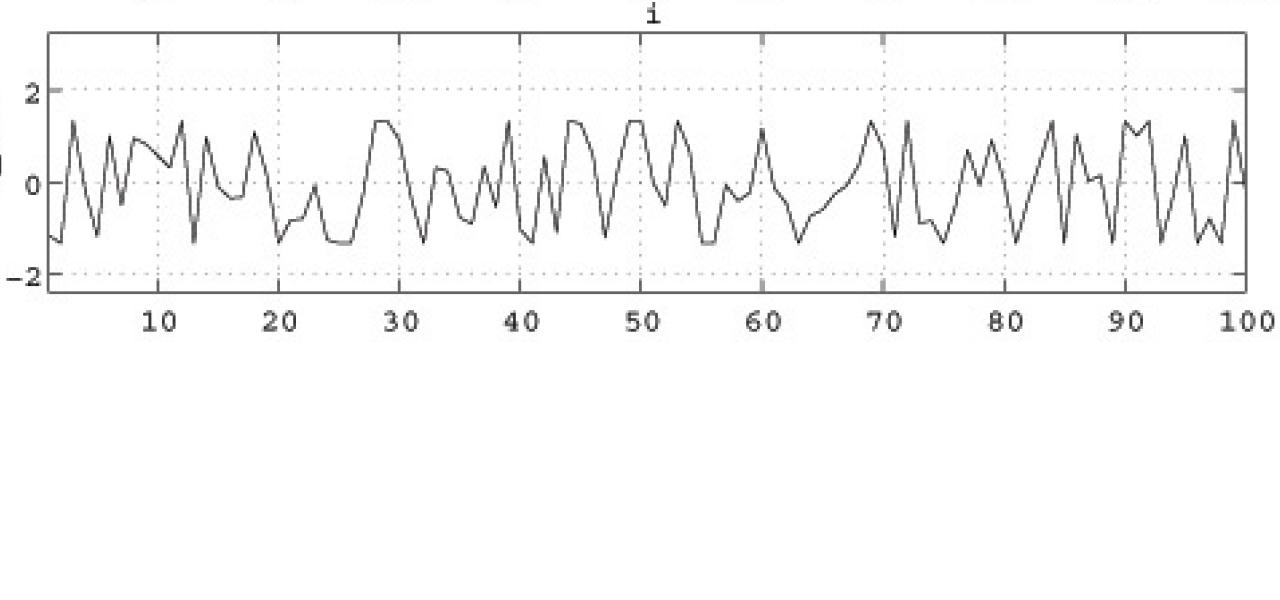
\includegraphics[scale=0.3]{residus.jpg}
    \end{center}

    \begin{solution}
      Le vecteur $b \notin \mathcal{C}(A) $ si et seulement si le nombre de
      contraintes est strictement supérieur au nombre de variables
      (en faisant l'hypothèse que les contraintes
      sont linéairement indépendantes).
      Pour plus d'explications, voir transparents CM 3.
    \end{solution}

  \item Vrai ou faux? Justifiez vos choix par quelques lignes, un contre-exemple ou un dessin. Soyez assez précis pour convaincre
    que vous ne devinez pas la réponse mais ne fournissez toutefois pas une justification formelle et détaillée.

    \begin{enumerate}

% polyhedron

      \item L'union de deux polyèdres est un polyèdre.

%\item The empty set is a polyhedron.

%extreme points

      \item Tout polyèdre $P$ peut être écrit sous forme géométrique $P=\{ {\bf x} \in {\bf R}^n: \bf A \bf x\geq \bf b\}$.

      \item Tout polyèdre $P$ peut être écrit sous forme standard
        $P=\{ {\bf x} \in {\bf R}^n: \bf A \bf x= \bf b, \bf x \geq 0\}$.


% \item L'ensemble $\{(x,y,z):x^2+y^2+z^2\leq 1\}$ est un polyèdre.

%\item A polyhedron in standard form always has an extreme point.

%\item A non-empty bounded polyhedra has at least one
%non-degenerate vertex.

%\item A point in a polyhedron in standard form can be expressed as
%a convex combination of the polyhedron vertices.

%\item Let $x_0$ and $x_1$ be two vertices of a polyhedron in ${\bf
%R}^n$ and let the polyhedron be defined by $m$ linear
%inequalities. Then here is a path from $x_0$ to $x_1$ along edges
%of the polyhedron that passes through at most $m^m$ edges.

%\item If there exists a vector $\bf q \neq \bf 0$ for which $\bf A
%\bf q=\bf 0$, then the polyhedron $\{\bf x: \bf A \bf x\geq \bf
%b\}$ doesn't have any vertex.

%\item Suppose that the polyhedron $\{{\bf x}: \bf A \bf x\geq \bf
%b\}$  is non-empty and bounded, then $\bf x = \bf 0$ is the only
%vector for which $\bf A \bf x = \bf 0$.

% solutions

      \item L'ensemble des solutions optimales d'un problème d'optimisation linéaire est un polyèdre.

%Consider the set $Q$ of optimal solutions to $\min \{ {\bf c}'
%{\bf x}: {\bf A} {\bf x} \geq {\bf b}, {\bf x} \in {\bf R}^n\}$.
%The set $Q$ is a polyhedron and its extreme points are extreme
%points of the polyhedron $\{{\bf x} \in {\bf R}^n: \bf A \bf x
%\geq \bf b\}$.

%\item A linear optimization problem may have exactly two optimal
%solutions.


%\item At an optimal solution of a linear optimization problem in
%${\bf R}^n$ there are $n$ active constraints.

      \item En toute solution optimale d'un problème d'optimisation linéaire de
        $n$ variables il y a au moins $n$  contraintes actives.


%\item Let $\bf x$ be a basic feasible solution associated with
%some basic matrix. If $\bf x$ is the unique optimal solution, then
%the reduced cost of every nonbasic variable is positive.

% simplex




%\item If a linear optimization problem has an unbounded optimal
%cost, then its dual is infeasible.


%\item If a linear optimization problem is infeasible, then its
%dual has unbounded optimal cost.


%\item L'optimisation linéaire permet de faire une régression linéaire minimisant la norme $||\cdot||_\infty$ des résidus.


    \end{enumerate}

    \begin{solution}
      \begin{enumerate}
        \item Faux, on sait qu'un polyèdre est convexe or
          $\{x | x \leq -1\} \cap \{x | x \geq 1\}$ n'est pas convexe.
        \item Vrai, c'est même sa définition.
        \item Faux, on sait qu'un polyèdre sous forme standard admet
          toujours un sommet alors qu'en général un polyèdre n'admet pas
          toujours un sommet.
          Par exemple, $\{(x_1,x_2) \in \R^2 | x_1 \geq 0\}$ n'admet
          pas de sommet. Il en pourra donc pas être écrit sous forme standard
          sans faire un changement de variable qui modifiera le polyèdre.
          Il ne faut d'ailleurs pas confondre ça avec le fait que tout
          problème d'optimisation linéaire peut s'écrire sous forme standard.
          Car ici, on accepte pas de changement de variable car ça
          modifie le polyèdre.
        \item Vrai. En effet, on ait que l'ensemble admissible $\mathcal{D}$
          est un polyèdre.
          L'ensemble des solutions qui ont un coût optimal
          \[ \{x | c^T x = z^*\} =
          \{x | c^T x \geq z^* \land (-c^T) x \geq -z^*\} \]
          est aussi un polyèdre.
          L'ensemble des solutions optimale est l'intersection des deux est
          donc aussi un polyèdre car l'intersection de deux polyèdres est
          un polyèdre.
        \item Faux.
          Il ne faut pas faire dire au théorème fondamental
          ce qu'il ne dit pas.
          Si l'ensemble admissible possède un sommet et que le coût
          optimal est fini,
          il \emph{existe} un sommet optimal mais
          toutes les solutions optimales ne sont
          pas spécialement des sommets.
          Par exemple, pour le problème d'optimisation linéaire suivant
          \begin{align*}
            \min x_1\\
            (x_1,x_2) & \geq 0
          \end{align*}
          la solution optimale $(0,0)$ est un sommet mais la solution
          optimale $(0,1)$
          n'en est pas une.
          $(0,1)$ serre d'ailleurs une seule contrainte,
          ce qui constitue un contre exemple car on a deux variables.
      \end{enumerate}
    \end{solution}

\end{enumerate}
